\documentclass[12pt]{report}

\title{Zero-Knowledge Authentication}
\author{Jakob Povšič}

\usepackage{listings}
\usepackage{amsmath}
\usepackage{tgschola}
\usepackage{amsfonts}
\usepackage{mathptmx}
\usepackage{graphicx}
\usepackage{hyperref}
\usepackage{fontspec}

\fontfamily{qcs}

\newcommand{\Mod}[1]{\ (\mathrm{mod}\ #1)}

\renewcommand{\thefootnote}{\fnsymbol{footnote}}
\newcommand{\genlegendre}[4]{%
  \genfrac{(}{)}{}{#1}{#3}{#4}%
  \if\relax\detokenize{#2}\relax\else_{\!#2}\fi
}
\newcommand{\legendre}[3][]{\genlegendre{}{#1}{#2}{#3}}
\newcommand{\dlegendre}[3][]{\genlegendre{0}{#1}{#2}{#3}}
\newcommand{\tlegendre}[3][]{\genlegendre{1}{#1}{#2}{#3}}

\begin{document}
\pagenumbering{Roman}

\maketitle
\newpage

\tableofcontents
\newpage

\pagenumbering{arabic}

\section*{Abstract} %TODO: Extend somehow
We design an authentication protocol that can be used to authenticate users over a network with a username and password.
The protocol uses the zero-knowledge proof (ZKP) of quadratic residuosity protocol as a verification mechanism.
It is designed on top of the Extensible Authentication Protocol (EAP) framework as an EAP method.
The ZKP verification protocol yields interesting security properties that make the protocol favourable to be used over insecure networks.

\newpage

\chapter{Introduction}


\section{Introduction} %TODO: Extend somehow
%Authentication is a core component of computer security and an indispensable part of our modern digital lives.
%In this thesis we design an authentication protocol using Zero-Knowledge Proofs (ZKPs), an interesting cryptographic phenomenon that can prove mathematical statements without revealing \textit{why} they are true.
%Our protocol enables network authentication using a username and password.
%To create a secure password authentication protocol we have to be aware of the common pitfalls  and how modern security systems handle them.
%We use the Extensible Authentication Protocol (EAP) as the framework on top of which we design our authentication protocol.
%
%\newpage

Our lives are becoming more digital everyday, and with big tech companies whose business models rely on user data, privacy is becoming an ever bigger issue.
Individuals participating in a digital spaces and keeping control of their personal data seem mutually exclusive terms today, however technologies like zero-knowledge proofs can help us achieve the seemingly impossible task.
Zero-knowledge proofs are a very interesting cryptographic phenomenon that can prove mathematical statements, without revealing \textit{why} they are true. This has incredibly interesting real world applications.

Cryptocurrencies Monero and Zcash are using zero-knowledge proofs to validate transactions on their networks while keeping transaction senders, recipients anonymous and amounts opaque.

The Self Sovereign Identity space is using zero-knowledge proofs and blockchain technologies to build a decentralised and privacy preserving digital identity infrastructure.
Zero-knowledge proofs enable asking complex questions about sensitive user credentials in a completely privacy preserving manner.
For example, proving you are over 18 without revealing your date of birth, or that you hold a certain amount of funds in your bank account without disclosing your financial statements.

Advancements like this hint that we will look at this time and our attitude to personal data handling, as we today look at feudalism.
\bigskip
\\
In this thesis we want to utilise zero-knowledge proofs in a password authentication protocols.
When creating a password authentication system we have to protect ourselves from password vulnerabilities, however the integration of key stretching methods is not as straight forward as in regular password authentication systems, because of the underlying zero-knowledge proof.
Our protocol is built on top of the extensible authentication protocol (EAP), an extensible authentication framework.

%TODO: Interesting story

%TODO: Work structure 

%
%In computer systems authentication is a process where a system user asserts their identity via an authentication method.
%There are many authentication systems appropriate for different use cases,
%one of the most common systems for end user authentication is a combination of username and password.
%
%
%Our authentication protocol is using zero-knowledge proofs (ZKP) to verify the users password. 
%ZKPs are proofs that prove noting more than that they are true, this allows us to verify the users password without ever revealing or sending the password or password equivalents over the network.
%
%Conceptually passwords are secrets memorised by the user, and it is often the case that weaker passwords are easier to memorise, additionally many users reuse passwords between different systems.
%When designing a password authentication system, we must keep adopt strategies that mitigate the vulnerabilities of passwords.
%
%
%Password authentication is based on a shared secret between the user and the system. Passwords however require special handling because 
%
%
%
%
%
%In computer systems authentication is a process where a system user asserts their identity.
%
%Extensible Authentication Protocol (EAP) is a general purpose authentication protocol framework, designed for network authentication.
%It defines a set of messages and communication patterns to support the negotiation and execution of authentication protocols.
%EAP is authentication method agnostic and is designed to be extended with new authentication methods.
%
%There are many types of authentication methods appropriate for different use cases and contexts, one of the most common authentication methods is a combination of username and password.
%
%In a secure implementation of a password authentication, the system needs protect itself from shortcomings for passwords.



%%Passwords
%One of the most common authentication use cases is end-user authentication with a username and password.
%
%To securely use password authentication, we have to adapt our system to work around short comings of passwords.
%
%%NIST
%Authentication protocols focus on execution in a context where all necessary data exists. 
%NIST Digital Identity Guidelines outline the complete lifecycle of an authentication system.
%
%%ZKP
%Zero-Knowledge Proofs are proofs that reveal only that something is true, without revealing why it is true.
%A simple ZKP protocol is for the problem of quadratic residuosity, which can be used as a basis for a password authentication protocol within the EAP framework.
%
%The protocol has to be extended to overcome the short comings of passwords.
%
%
%
%
%* Authentication
%* Password authentication
%* EAP
%* ZKP







%TODO: Move to ZKP section


%TODO: Add VC in-range/in-set ZKPs

\newpage

\chapter{Methodologies and Tools}
\section{Authentication}

Authentication the process of proving a claim or an assertion.
Today it is most commonly used in information security, however methods of authentication are not limited to computer science and are also used in fields of archeology, anthropology and others.
\bigskip
\newline
In computer science authentication is used for establishing access between restricted system resources and users through digital identities.
Government and international institutions have developed guidelines for managing digital identities and authentication processes \cite{grassi2017} .
\bigskip
\newline %TODO: Remove
While both humans and other computer systems can be authenticated, we are focusing on how authentication of a human end user.




\subsection{Authentication Process Components}
Authentications is a method used in information security to manage access between restricted system resources and an external user or system wishing to access them.

As defined in RFC-4949 \cite{shirey2007internet}, authentication is \textit{the process of verifying a claim that a system entity or system resource has a certain attribute value.}
This is a broad definition, and it most frequently applies to the verification of users identity (e.g at login), however assertions can be made and verified about any subject or object.
The process of authentication is done in two parts, \textit{identification} and \textit{verification}.

\paragraph{Identification} Presenting an identifier to the authentication system, that establishes the entity being authenticated, this is commonly a username or an email address.
The identifier needs to be unique for the entity it identifies.

The process of identification is not necessarily externally visible, as the identity of the subject/object can be implicit from the user context. 
For example an identifier can be determined by an IP address the user wants to authenticate from, or a system might only have a single identity that can authenticate.

\paragraph{Verification} Presenting or generating authentication information that can be used to verify the claim.
Commonly used authentication information are passwords, one-time tokens, digital signatures.

\subsection{Authentication Factors}

As described in \cite{council2005authentication} authentication systems can rely on three distinct "factors".

\begin{itemize}
	\item \textbf{Knowledge factors} - Something the user \textbf{knows} (e.g, password, security question, PIN)
	\item \textbf{Ownership factors} - Something the user \textbf{owns} (e.g, ID card, security tokens, mobile devices)
	\item \textbf{Inherence factors} - Something the user \textbf{is} or \textbf{does} (e.g, static biometrics - fingerprints, retina, face. dynamic biometrics - voice patterns, typing rhythm)
\end{itemize}

\paragraph{Strong authentication} As defined by governments and financial institutions \cite{schaeffer2010national, ecb2013recommendations}, secure authentication is based on two or more authentication factors. 
This is also referred to as \textit{multi-factor authentication}.

\newpage
\section{Password Authentication}

Passwords are one of the most common and oldest forms of user authentication, being first used in computers at MIT in the mid-60s \cite{mcmillan2012password}.

We need to understand the high level model of password authentication, pitfalls and solutions to overcome them.

\subsection{Authentication Model}

% High level arch
Password based authentication is a simple model, based on a shared secret (called a password) between a user and a system.
The password is often used in a combination with a user ID. 
The password is usually a set of characters or words memorised by the user, inputted via a keyboard.

To authenticate the user exchanges the password with the system, and the system authenticates the user according to passwords validity.

\begin{figure}[h]
	\centering
	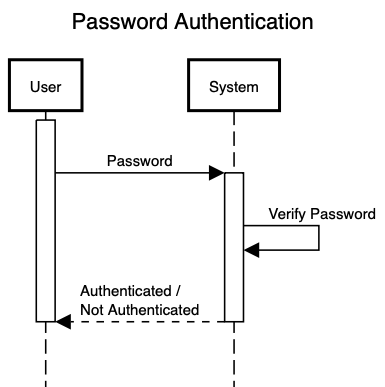
\includegraphics[height=8cm]{images/password-authentication}
	\caption{Password Authentication Model}
	\label{fig:password-authentication}
\end{figure}

\subsection{Security Vulnerabilities}
\label{label:password-vulnerabilities}

In a common password authentication system implementation used on the web, the user sends a plain-text password over a secure HTTPS connection, the server verifies it and responds.
The simplicity that makes passwords practical for users is what makes them especially vulnerable for systems that use them.

Because passwords are supposed to be memorised and the proliferation of websites requiring them, users tend to pick password that are easier to remember and reuse passwords across different websites \cite{conklin2004password}.
Many websites also don't properly handle passwords, enabling attackers to access plain-text passwords when a security breach happens.
The industry is aiming to improve password security with the adoption of password managers and initiatives like FIDO \cite{balfanz2013fido} working to retire passwords altogether.

Attacks can be according to NIST \cite{grassi2017} classified as \textit{online} or \textit{offline}, based on wether the attacker is directly interacting with an authentication system.

\subsubsection{Online Attacks} An attack where an attacker is directly interacting with the system.
These attacks are usually very \textit{noisy}, making it easy for an authentication system to detect an attack is happening and react. For this reason, most online attacks are not very effective.
For example, locking an account after 5 failed authentication attempts.

Effective online attacks work by operating under the radar of detection, for example, by trying out a small number of passwords on each user.
Popular methods are \textit{password spraying} and \textit{credential stuffing} \cite{haber2020attack}, both of which utilise information from data breaches, like lists of most commonly used passwords, or username and password combinations.
\textit{Password spraying} is taking a small number of commonly used passwords and attempting to authenticate with a large number of accounts, the attacker is assuming that in a large sample of accounts some will be using common passwords.
\textit{Credential stuffing} is taking a compromised user credential, for example a username and password combination found in a data breach, and using them to authenticate into multiple websites. 
The attacker is assuming that if a person is using a set of credentials on one website, they are potentially reusing them on other websites.

\subsubsection{Offline Attacks}
Is an attack performed in a system controlled by the attacker.
For example, an attacker might analyse data on his personal computer to extract sensitive information.
The data is obtained by either theft of file, eavesdropping an authentication protocol or a system penetration.

\textit{Password cracking} \cite{blocki2018economics} is method of extracting user credentials from data used by the authentication system to verify users credentials.
The success of password cracking is generally determined by two parameters, the time required to check a single password and number of guesses required or the strength of the underlying password.

\subsubsection{Security Practices}
\label{password-security-practices}
There are many different things an authentication system can incorporate to improve its security.
An authentication system can adopt techniques for preventing active attacks and improving password strength without affecting the underlying zero-knowledge  protocol.
We are going to be focusing on methods for handling passwords on the data layer, where we protect ourselves against offline attacks.
The form in which passwords exits on the data layer is also constrained by the ZKP protocol used for password verification.

\paragraph{Key-Stretching}
\label{paragraph:password-hashing}
Protecting passwords on the data layer is of critical importance.
\textit{Key-stretching} \cite{hornby2016salted} also called \textit{password hashing} is the industry standard method of improving security of low entropy secrets like passwords.

%An insecure system might store the passwords or password-equivalent data in plain text and compare them for verification. While simple, this system is insecure as user credentials directly are exposed with any unauthorised access.x
With this approach the password $p$ is \textit{stretched} or "hashed" using a function $H$ and a high entropy value called a \textit{salt} $s$, the output called a \textit{password hash} $p_H$ and the salt are stored in persistent memory while the plain text password is discarded.
$$H(p, s) = p_H$$

When verifying the password $p'$, it is stretched again with the stored salt $p$ and the output hash $p{'}_H$ is compared with the stored password hash $p_H$, if it matches the password is correct.
$$H(p', s) = p{'}_H$$
$$p{'}_H \stackrel{?}{=} p_H$$

Key-stretching \cite{blocki2018economics} is traditionally done with hash iteration functions (PBKDF2, BCRYPT), these algorithms are CPU intensive, however are vulnerable to attackers with special purpose hardware (ASIC), so a better choice are memory-hard algorithms (Argon2, Scrypt, Balloon) \cite{biryukov2016argon2, percival2016scrypt, boneh2016balloon}.\\
%Because salt is stored alongside password hashes, systems sometimes also utilise a third value called \textit{pepper}, which is the same for all passwords, but stored in a different place from the salt.
%\newline
%When using a key stretching method with a function $H$, the password $p$ is stretched with a salt $s$, the password hash $p_H$ and salt $s$ are stored, while the password $p$ can be discarded.
%When authenticating the user, the system stretches the submitted password $p'$ with the stored salt $s$, and compares the hash $p{'}_H$ with the stored hash $p_H$ to know if the password is correct.
%
%

%\subparagraph{Password Strength}
%Measure of entropy with determines the difficulty of the password being guessed.
%Re-using passwords greatly undermines password strength and is what attacks like credential stuffing rely on.
%Have I Been Pwned \cite{hunt2021have} catalogs 613,584,248 passwords recovered from data breaches, while CrackStation \cite{hornby2019password} lists a collection of 1,493,677,782 words used for password cracking.
%Some papers \cite{blocki2018economics} have provided strong evidence that passwords follow a Zipf's law distribution.
\section{Extensible Authentication Protocol}
\label{section:eap}
Our protocol should be implemented using the EAP framework, lets overview how the protocol works and how we were to implemented a new EAP method.


%EAP - PROTOCOL IN DETAIL

\subsection{Overview}
Extensible Authentication Protocol \cite{aboba2004extensible} (EAP) is a general purpose authentication framework, designed for network access authentication, where IP might not be available. 
It runs directly over the data link layer such as PPP  \cite{simpson1994rfc1661} and IEEE 802.

EAP defines a set of messages that support negotiation and execution of a variety of authentication protocols.

EAP is a two-party protocol between a \textit{peer} and an \textit{authenticator} at the each end of a link. The terms \textit{peer} and \textit{authenticator} are EAP terminology.
In the protocol the peer is authenticating with the authenticator.

\subsection{Messages}
The peer and the authenticator communicate by exchanging \textit{EAP messages}.
The protocol starts with the authenticator sending a message to the peer, they keep exchanging messages until the authenticator can either authenticate the peer or not.

Messages are exchanged in a lock-step manner, where an authenticator sends a message and the peer responds to it. 
The authenticator dictates the order of messages, meaning it can send a message at any point of communication, as opposed to the peer, which can only respond to messages from the authenticator.
Any messages from the peer not in a response to the authenticator are discarded.

\begin{figure}[h]
	\centering
	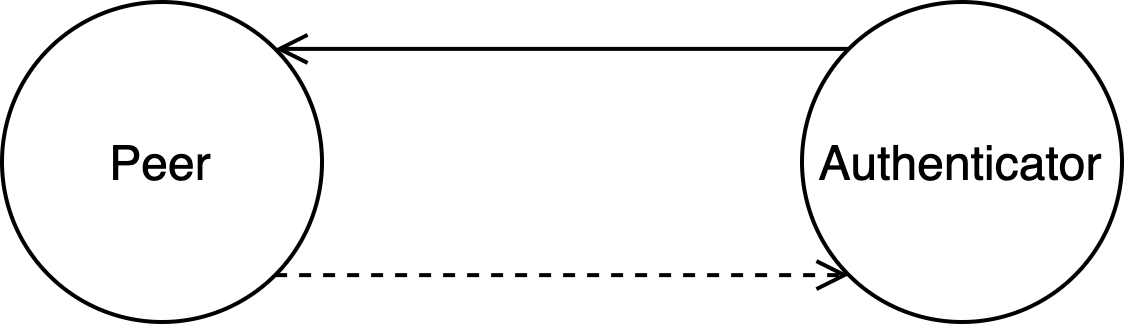
\includegraphics[width=8cm]{images/eap-messages}
	\caption{Peer and Authenticator Communication}
	\label{fig:eap-messages}
\end{figure}

\subsubsection{EAP Message Structure}
Messages are composed of fields, each field length is multiple of an octet of bits.
Each field type has a special purpose in EAP.

\begin{center}
	\begin{tabular}{|c|c|c|c|c|c|}
		\hline
		Length (Octets) & 1 & 1 & 2 & 1 & $n \le 2^{16}$\\
		\hline
		Field Type & Code & Identifier & Length & Type & Type-Data\\
		\hline
	\end{tabular}
\end{center}

%TODO: EAP Packet with table

\subsubsection{Code Field}
The code field determines who the packet is intended for and how or even should the recipient respond.

\begin{description}
	\item[Request]\textit{Code 1}. Messages sent by the authenticator to the peer.
	\item[Response]\textit{Code 2}. Messages sent by the peer to the authenticator as a reply to a \textit{request} message.
	\item[Success]\textit{Code 3}. Sent by the authenticator, after the peer is successfully authenticated. The peer doesn't have to respond to the message.
	\item[Failure]\textit{Code 4}. Sent by the authenticator, if the peer cannot be authenticated. The peer doesn't have to respond to the message.
\end{description}

\subsubsection{Identifier Field}
The identifier field is used to match request and response messages, each response message needs to have the same identifier as the request.
The authenticator will discard response messages that don't have a matching identifier with the current request.
The peer does not re-transmit response message, but relies on the authenticator to re-transmit a request message after some time if the matching response is lost.

\subsubsection{Length Field}
The length field determines the total size of the EAP message. Because EAP provides support for generic authentication methods, the final length of the messages is variable.
The length of the Type-Data field is entirely dependent on the authentication method used.

%EAP - METHODS

\subsubsection{Type and Type-Data Field}
The \textit{type} field determines how the message should be processed and how to interpret the \textit{type-data} field.
Most message types represent authentication methods, except four special purpose types.

The \textit{type} used is determined by the authenticator when sending the request message. The response message from a peer needs to be of the same \textit{type} as the request, except in cases where that \textit{type} is not supported by the peer.

\begin{description}
	\item[Identity] \textit{Type 1}. Used to query the identity of the peer. The type is often used as an initial message from the authenticator the peer, however its use is entirely optional and EAP methods should rely on method-specific identity queries.
	
	\item[Notification]\textit{Type 2}. Used to convey an informative message to the peer, by the authenticator. Usage of this type is entirely optional.
	\item[Nak]\textit{Type 3}. Used only as a response to a request, where the desired type is not available.
	The peer includes desired authentication methods, indicated by their type number.
	This type is also referred to as Legacy Nak, when compared to \textit{Expanded Nak} (sub-type of the Expanded Type).
	\item[Expanded Type] \textit{Type 254}. 
	Used to expand the space of possible message types beyond the original 256 possible types.
	The expanded type \textit{data field} is composed from a \textit{Vendor-ID} field, \textit{Vendor-Type} and the type data.
	\bigskip
	\begin{center}
		\begin{tabular}{|c|c|c|c|c|c|}
		\cline{2-5}
		\hline
		Length (octets) & & 3 & 4 & n\\
		\hline
		Type Field & ... & Vendor-ID & Vendor-Type & Vendor-Type Data\\
		\hline
		\end{tabular}
	\end{center}
	\bigskip
	A peer can respond to an unsupported request type with an \textit{expanded nak}, if he desires to use an EAP method supported with the expanded type.
	\item[Experimental] \textit{Type 255}. This type is used for experimenting with new EAP Types and has not fixed format.
\end{description}

\subsubsection{Authentication Methods}
The remaining types correspond to different authentication methods.
In IANA \cite{joseph2004eap} 49 authentication methods have been assigned type numbers.
The original RFC \cite{aboba2004extensible} already assigned 3 authentication protocols.

\begin{description}
	\item[MD5-Challenge] \textit{Type 4}. An EAP implementation of the \cite{simon2008eap} PPP-CHAP protocol.
	\item[One-Time Password] \textit{Type 5}. An EAP implementation of the \cite{haller1998one} one-time password system.
	\item[Generic Token Card] \textit{Type 6.} This type facilitates various challenge/response \textit{token card} implementations.
\end{description}

Some other notable examples are EAP-TLS \cite{simon2008eap}, EAP-PSK \cite{bersani2007eap}.
EAP SRP-SHA1 \cite{carlson135eap} is especially interesting as it uses a zero-knowledge protocols to verify the peers secret.

\subsection{Pass-Through Behaviour}
An authenticator can act as a \textit{Pass-Through Authenticator}, by using the authentication services of a \textit{backend authentication server}.
In this mode of operation the authenticator is relaying the EAP messages between the peer and the backend authentication server.
For example, in IEEE 802.1x the authenticator communicates with a RADIUS server \cite{congdon2003ieee}.

\paragraph{IEEE 802.1x}

Is a port based network access control standard for LAN and WLAN.
It is part of the IEEE 802.11 group of network protocols.

IEEE 802.1x defines an encapsulation of EAP for use over IEEE 802 as EAPOL or "EAP over LANs".
EAPOL is used in widely adopted wireless network security standards WPA2. 
In WPA2-Enterprise, EAPOL is used for communication between the supplicant and the authenticator.

With WPA2-Enterprise, the authenticator functions in a pass-through mode and uses a RADIUS server to authenticate the supplicant.
EAP packets between the authenticator and the authentications server (RADIUS) are encapsulated as RADIUS messages \cite{aboba2003radius, chen2005extensible, congdon2003ieee}
\section{Zero-Knowledge Proofs}

\subsection{Introduction}

Traditional theorem proofs are logical arguments that establish truth through inference rules of a deductive system based on axioms and other proven theorems.
\textit{Zero-Knowledge Proofs} (ZKPs) are compared to traditional proofs probabilistic meaning they \textit{"convince"} the verifier with a small margin of error.

They were first defined by Goldwasser, Micali and Rackoff in \cite{GMR} in a paper published in 1985. 
They proposed a proof system as a two-party protocol between a \textit{prover} and a \textit{verifier}. 
It relies on the computational difficulty of the quadratic residuosity problem (QRP).

\subsubsection{The Strange Cave of Ali Baba}
A famous example of a zero-knowledge proof protocol made by \cite{QJM} is The Strange Cave of Ali Baba.

\begin{figure}[h]
	\centering
	\includegraphics[height=6cm]{images/zkp}
	\caption{The Strange Cave of Ali Baba}
	\label{fig:strange-cave-of-alibaba}
\end{figure}

\bigskip

Ali Baba's cave has a single entrance, that splits into two tunnels that meet in the middle where there is a door that can only be opened with a secret passphrase.

\bigskip

Peggy (or Prover) wants to prove to Victor (or Verifier) that she knows the secret passphrase, but she doesn't want to revel the secret nor does she want to reveal her knowledge of the secret to anyone else besides Victor.

\bigskip

To do this they come up with a scheme.
Victor turns away from the entrance of the cave, so he cannot see Peggy, as she enters the cave and goes into one of the tunnels at random. 
Victor then turns around and tells Peggy which tunnel to come out of.
Peggy knowing the secret can pass through the door in the middle and emerge from the tunnel requested.

\bigskip

If Peggy didn't know the secret she could still convince Victor, by entering the correct tunnel by luck.
But since Victor is choosing the tunnel at random, Peggy's chance of picking the correct tunnel is 50\%. If Victor were to repeat the process $n$ time, her chances of fooling him become arbitrarily small ($2^{-n}$).

With this process Victor can be convinced that Peggy really knows the secret with a very chance ($1 - 2^{-n}$).

\bigskip

Further more any third party observing the interaction cannot be convinced of the validity of the proof because it cannot be assured that the interaction was truly random. 
For example, Victor could have told Peggy his questions in advance, so Peggy would produce a convincing looking proof.

%There are three main ingredients that make interactive zero-knowledge proofs work. %TODO: Move this part to the end of the section
%
%\begin{enumerate}
%	\item Interaction - The prover and the verifier exchange messages back and forth.
%	\item Hidden Randomisation - The verifier relies on randomness that is hidden from the prover, and thus unpredictable from him.
%	\item Computational Difficulty - The prover embeds his proof in computational difficulty of some other problem.
%\end{enumerate}

\subsection{Applications}
Most commonly ZKPs were used in authentication and identification systems, as a way to prove knowledge of a secret. 
Recently however there have been a number of new applications in the cryptocurrency and digital identity spaces.

The cryptocurrency Zcash uses a \textit{non-interactive zero-knowledge protocol} zk-SNARK \cite{bowe2018multi} to prove the validity of transactions, without revealing anything about the recipients nor the amount sent.

The cryptocurrency Monero uses a ZKP protocol Bulletproofs \cite{bunz2018bulletproofs}, to achieve anonymous transactions.

\textit{Idemix} \cite{camenisch2002design} an anonymous credential system for interaction between digital identities relies on CL-signatures \cite{camenisch2001efficient} to prove ownership of a credential offline, without the issuing organisation.
Idemix has been implemented in the open-source Hyperledger Indy project.

\subsection{Interactive Proof Systems}
\textbf{Interactive proof systems} are proof systems between a prover and a verifier, which exchange messages to decide on the validness of the proof.
The prover is a computationally unbounded polynomial time Turing machine and the verifier is a probabilistic polynomial time Turing machine.


The properties of \textit{completeness} and \textit{soundness} define an interactive proof system.

\paragraph{Completeness}

Any honest prover can convince the verifier with overwhelming probability.\\
For each $k \in \mathbb{N}$ and sufficiently large $n$;

$$\Pr[x \in L; P(x) = y; V(y) = 1] \ge 1 - \frac{1}{n^k}$$

\paragraph{Soundness}

Any verifier following the protocol will reject a cheating prover with overwhelming probability.\\
For each $k \in \mathbb{N}$ and sufficiently large $n$;

$$\Pr[x \notin L; P(x) = y; V(y) = 0] \ge 1 - \frac{1}{n^k}$$


\subsubsection{Interactive Polynomial Time Complexity}
Any problem solvable by an interactive proof systems is in the class of \textbf{IP}.

\subsubsection{Other Variants of Interactive Proof Systems}

\paragraph{Arthur-Merlin protocol} Problems in the class \textbf{AM}, an Arthur-Merlin protocol \cite{babai1985trading} is an interactive protocol similar to IP, with the difference in that its a \textit{public-coin protocol}. 
Meaning that verifiers internal state is visible to the prover, while in IP the state is hidden.
%I has been proven that AM is equally powerful as IP and that AM's public internal state gives the prover no advantage. %TODO: Add citation

\paragraph{Multi Prover Interactive Proofs}
\textbf{MIP} \cite{ben2019multi} is a more powerful model, utilising two provers that communicate with a single verifier.
This models has been build to address the shortcomings of IP.
MIP proved that every problem has a ZKP system, without the assumption that one-way functions exist.

\subsection{Knowledge Complexity}

\textit{Zero-knowledge proof systems} prove the  membership of $x$ in language $L$, without revealing any additional knowledge (e.g why is $x \in L$).

The essence of zero-knowledge is the idea that what the verifier \textit{sees} is indistinguishable from what can be easily \textit{simulated} on public inputs.
The term \textit{knowledge complexity} quantifies the degrees of indistinguishability of different languages and proof constructions. 

\subsubsection{Indistinguishability}
Indistinguishability describes degrees of an ability to distinguish between two random variables $U, V$.
\bigskip
\newline
Let $U = \{U(x)\}$ and $V = \{V(x)\}$ be two families of random variables, where $x$ is from a language $L$, a subset of $\{0, 1\}^*$.
\newline
An algorithm $A(x)$ is given a random sample $x$ from either distribution and will output either $1$ or $0$, depending which distribution it determines the sample originated from.
Distributions become "indistinguishable" as the outputs of the algorithm become uncorrelated to the origin of the sample.

By bounding the \textit{size} of the sample and the \textit{time} given to the algorithm we can obtain different notions of indistinguishability.

%\subsubsection{Indistinguishability of Random Variables} %TODO: Simplify this
%
%Let $U = \{U(x)\}$ and $V = \{V(x)\}$ be two families of random variables, where $x$ is from a language $L$, a particular subset of $\{0, 1\}^*$.
%
%In the framework for distinguishing between random variables, a "judge" is given a sample selected randomly from either $V(x)$ or $U(x)$.
%A judge studies the sample and outputs either a $0$ or a $1$, depending on which distribution he thinks the sample came from.
%
%$U(x)$ essentially becomes "replaceable" by $V(x)$, when $x$ increases and any judges prediction becomes uncorrelated with the origin distribution.


\paragraph{Equality} 
%Given that $U(x)$ and $V(x)$ are equal, they will remain indistinguishable, even if the samples are of arbitrary size and can be studied for an arbitrary amount of time.

If $U(x)$ and $V(x)$ are equal, outputs of a computationally unbounded algorithm will remain uncorrelated with the origin of the sample.

\paragraph{Statistical Indistinguishability} Two random variables are statistically indistinguishable, when the algorithms outputs remain uncorrelated with the origin, given an arbitrary amount of time and a poly-bounded sample size.
\bigskip
\newline
Let $L \subset \{0,1\}^*$ be a language, $U(x)$ and $V(x)$ are statistically indistinguishable on $L$ if,
\bigskip
$$|\Pr [A(x, U) = 1] - \Pr [A(x, V) = 1]| < |x|^{-c}$$ %TODO: Probably not right, check later.
\bigskip
\newline
for $\forall c > 0$, and sufficiently long $x \in L$. 

%\subparagraph{Statistical Indistinguishability} Two random variables are statistically indistinguishable, when given a polynomial sized sample and an arbitrary amount of time, the judges verdict remains meaningless.
%
%\bigskip
%
%Let $L \subset \{0,1\}^*$ be a language, $U(x)$ and $V(x)$ are statistically indistinguishable on $L$ if,
%
%$$\sum_{\alpha \in \{0,1\}^*} |prob(U(x) = \alpha) - prob(V(x) = \alpha) | < |x|^{-c}$$
%
%
%
%for $\forall c > 0$, and sufficiently long $x \in L$. 

\paragraph{Computational Indistinguishability} %TODO: Probably need to clarify the link between poly-time algorithm and poly-sized family of circuits.
Two random variables are computationally indistinguishable, when the poly-time bounded algorithms outputs remain uncorrelated with the origin, given a poly-bounded sample size.
\bigskip
\newline
Let $L \subset \{0,1\}^*$ be a language, poly-bounded families of random variables $U(x)$ and $V(x)$ are computationally indistinguishable on $L$ if for all poly-sized family of circuits $C$, $\forall c > 0$, and a sufficiently long $x \in L$

$$|\Pr[C(U, x) = 1] - \Pr[C(V, x) = 1]|  < |x|^{-c}$$


%\subparagraph{Computational Indistinguishability}%TODO: Simplify this
%
%Two random variables are computationally indistinguishable, if judges verdict remains meaningless given a polynomial sized sample and polynomial amount of time.
%
%\bigskip
%
%Let $L \subset \{0,1\}^*$ be a language, poly-bounded families of random variables $U(x)$ and $V(x)$ are computationally indistinguishable on $L$ if for all poly-sized family of circuits $C$, $\forall c > 0$, and a sufficiently long $x \in L$
%
%$$|P(U, C, x) - P(V, C, x)| < |x|^{-c}$$
%
%Any two families that are \textit{computationally indistinguishable} are considered  \textit{indistinguishable} in general.

\subsubsection{Approximability of Random Variables}%TODO: Simplify this

The notion of approximability described the degree to which a random variable $U(x)$ can be "generated" by a probabilistic Turing machine $M$, generating a probability distribution $M(x)$.
\bigskip
\newline
A random variable $U(x)$ is \textit{perfectly approximable} if there exists a probabilistic Turing machine $M$, such that for $x \in L$, $M(x)$ is \textit{equal} to $U(x)$.
\newline
$U(x)$ is statistically or computationally approximable if $M(x)$ is statistically or computationally indistinguishable from $U(x)$.

\bigskip

Generally speaking when saying a family of random variables $U(x)$ is \textit{approximable} we mean that it is \textit{computationally} approximable.

\subsubsection{Definition of Zero-Knowledge}

Zero-knowledge is a degree of protocols knowledge complexity at which no meaningful information can be extracted by the verifier or any third party observer.
\bigskip
\newline
A protocol is zero-knowledge if the verifiers "view" is approximable by a simulator $S$.
A verifiers view is all data that was exchanged with the prover, a cheating verifier's view might have extra information (e.g a history of previous interactions).

A protocols is perfectly zero-knowledge if the view is perfectly approximable for all verifiers.
Statistical or computational zero-knowledge is obtained by statistical or computational approximability.
\section{Languages with Zero-Knowledge Proof Systems}
The zero-knowledge property of interactive proofs is determined by the language the proof exists for.
The choice of language also determines the ZKPs practical applicability.
\bigskip
\newline
The original ZKP protocols \cite{GMR} were proposed for the languages of Quadratic Residuosity problem (QRP) and Quadratic Non-Residuosity Problem (QNRP).
Other simpler protocols are also based on the Discrete Logarithm problem \cite{wu1998secure} and Graph Isomorphism Problem \cite{goldreich2019proofs}.

It has been proven in \cite{GMW} that every language in \textbf{NP} has a ZKP system.

ZKP and interactive protocols have also been used as a tool for studying language complexity \cite{shamir1992ip}.
\bigskip
\newline
In this thesis we are focusing the language QRP.

\subsection{Zero-Knowledge Proof of Quadratic Residuosity Problem}
\textit{Quadratic Residuosity Problem} was used in the original ZKP protocol in the founding paper \cite{GMR}. QRP has a \textit{perfect} zero-knowledge proof system.

QRP is much older than the \cite{GMR} paper, it was first described by Gauss in 1801 \cite{gauss1801disquisitiones}.

\subsubsection{Quadratic Residues} \cite{andrews1994number}
Quadratic residues come from modular arithmetic, a branch of number theory.
\bigskip
\newline
For $a, n \in \mathbb{Z}$, $n > 0$, $\gcd(a, n) = 1 $.
$a$ is a \textit{quadratic residue} if  $\exists x:x^2 \equiv a \Mod{n}$, otherwise $a$ is a \textit{quadratic non-residue}.
\bigskip
\newline
When $n$ is an odd prime, $a$ is a quadratic residue modulo $n$, if and only if.

$$a^{\frac{n-1}{2}} \equiv 1 \Mod{n}$$

\paragraph{Legendre Symbol}
$\dlegendre{a}{p}$ simplifies computations with quadratic residues.
\bigskip
\newline
If $p$ is an odd prime then,

\begin{center}
	$\dlegendre{a}{p} =
		\begin{cases}
			1 & \text{if $a$ is a quadratic residue modulo $p$}\\
			0 & \text{if p $\arrowvert$ a}\\
			-1 & \text{otherwise}
		\end{cases}$
\end{center}

\paragraph{Jacobi Symbol}
A generalised definition of the Legendre symbol $\dlegendre{a}{m}$, to allow the case where $m$ is any odd number.

If $m = p_1p_2 \cdots p_n$, where $p_i$ are odd primes, then
$$\dlegendre{n}{m} = \dlegendre{n}{p_1}\dlegendre{n}{p_2} \cdots\dlegendre{n}{p_n}$$

\subsubsection{Prime Factorization}
\cite{andrews1994number} The \textit{Fundamental Theorem of Arithmetic} states that for each integer \newline $n > 1$, exist primes $p_1 \le p_2 \le \cdots \le p_r$, such that $n = p_1 p_2 \cdots p_r$.
\bigskip
\newline
The process of prime factorization is a decomposition of a number $n$ to its prime factors $p_1 p_2 \cdots p_r$.

Currently no efficient algorithm exists for prime factorization. The problem is especially hard when factoring \textit{semiprimes}, a product of two prime numbers.
This hardness of this problem is used as a core building block in modern asymmetric cryptography like RSA \cite{rivest1978method}.


\subsubsection{Quadratic Residuosity Problem}
Given $a$, semiprime $n = pq$, where $p$ and $q$ are unknown different primes, and Jacobi symbol $\dlegendre{a}{n} = 1$.
\newline
Determine wether $a$ is a quadratic residue modulo $n$ or not.
\bigskip
\newline
The Jacobi Symbol can be efficiently computed using the \textit{Law of Quadratic Reciprocity}, but it does not always tell us if $a$ is quadratic residue modulo $n$ or not. 

$$\dlegendre{a}{n} =\dlegendre{a}{p}\dlegendre{a}{q}$$
If $\legendre{a}{n} = 1$ then $a$ is a quadratic residue both modulo $p$ and $q$, or $a$ is a quadratic non-residue both modulo $p$ and $q$.
To know wether $a$ is a quadratic residue modulo $n$ or not, we would have to know the prime factorization $p, q$ of $n$.
\newline
If $\legendre{a}{n} = -1$ we know $a$ is a quadratic non-residue modulo $p$ or $q$.


\subsubsection{ZKP Protocol for the Quadratic Residuosity Problem}

\begin{center}
	\begin{tabular}{rl}
		$n$ & Semiprime, where $\legendre{x}{n} = 1$\\
 		$x$ & Public input, where $x = w^2 \Mod n$\\
 		$w$ & Provers private input\\
	\end{tabular}
\end{center}


\begin{center}
	\begin{tabular}{r|c|l}
		Prover && Verifier\\
		\hline
		$u \leftarrow \Bbb{Z}_{n}^{*}; y = u^2 \Mod n$ & $\xrightarrow{y}$\\
		& $\xleftarrow{b}$ & $b \leftarrow_R \{0, 1\} $\\
		$z = uw^b\Mod n$ & $\xrightarrow z$ & verify $z^2 = yx^b \Mod n$\\
	\end{tabular}
\end{center}
This protocol is repeated $m$ times, for a probability of error of $\frac{1}{2^m}$.

\subsection{Computational Complexity Classes}

\subsubsection{Non-deterministic Polynomial Time}

\textbf{NP} is a class of problems solvable by a non-deterministic Turing machine in polynomial time. 
Or rather proof of any language in NP can be verified by a deterministic Turing machine in polynomial time.
\bigskip
\newline
Article \cite{GMW} proved that every language in NP has a zero-knowledge proof system, by creating a ZKP protocol for the Graph 3-Colouring problem (3-COL).

\textit{Minimum Colouring Problem} is a problem in graph theory, of what is the minimal $k$ \textit{proper} colouring of a graph, where no adjacent vertices are the same colour.
An instance of ($k=3$) colouring (3-COL) is proven to be \textit{NP-Hard} because a polynomial reduction exists from \textit{Boolean-Satisfiability problem} (3-SAT) to 3-COL \cite{mouatadid2014introduction}.
According to Cook's theorem \cite{cook1971complexity} 3-SAT is \textit{NP-Complete}, and any language in $L \in NP$ can be reduced to and instance of 3-SAT. 
Furthermore because polynomial reductions are \textit{transient}, any language $L \in NP$ can be reduced to an instance of 3-COL.

\subsubsection{Bounded-Error Probabilistic Polynomial Time Languages}

\textbf{BBP} is a class of problems that can be verified by a probabilistic Turing machine in polynomial time.

Trivially every language in BPP has a ZKP system, where the prover sends nothing to the verifier, the verifier checks the proof of $x \in L$ and outputs a the verdict. %TODO: Reword?

\subsection{Alternative Composition of Zero-Knowledge Proofs}
Zero-Knowledge Proofs can alternatively be composed in parallel as compared to sequential composition in \cite{GMR}.
Parallel composition is very interesting practically as it can help reduce the inefficiencies of communication between the prover and the verifier, especially over high latency networks.
\bigskip
\newline
In \cite{goldreich1996composition} they proved that only languages in BPP have 3-round interactive proofs that are zero-knowledge.

The QRP is not believed to be in BPP, so a parallel composition of QRP has weaker notion of zero-knowledge.




\chapter{Results}
\section{Protocol Design}
\label{label:protocol-design}
The main goal of our authentication protocol was to enable password authentication using zero-knowledge proof based on the quadratic residuosity problem. 
The computations used to assert the zero-knowledge proof present a vulnerability when used with passwords.
We extend the protocol with key stretching to protect the low entropy passwords.
The integration of key stretching is not as trivial as it might seem because of the underlying zero-knowledge protocol. 
We can overcome mathematical limitations imposed by the ZKP protocol by separating the data layer where all key stretching operations are done before the ZKP protocol.

In this section we will refer to the \S\ref{zkp-qrp} ZKP protocol of quadratic residuosity as the \textit{original protocol}  and our new protocol as the \textit{extended protocol}.

\subsection{Vulnerabilities}
Our use case is for password authentication, which features unique vulnerabilities, resulting from properties of passwords themselves, we've explored this topic in \S \ref{label:password-vulnerabilities}.
In particular the original protocol is vulnerable to offline attacks with pre-computed tables.
This vulnerability is caused the operation $x = w^2 \Mod{n}$ used to derive the quadratic residue $x$ mod $n$, which we later prove as a quadratic residue by proving the knowledge of secret $w$.
Intuitively the computation of this equation is relatively inexpensive when compared to special key-stretching function like \textit{Argon2} \cite{biryukov2016argon2}, allowing an attacker to use a pre-computed hash table or a rainbow table.

\newpage
\subsection{Limitations}
The solution seems to be a key stretching, as we've described in \S\ref{paragraph:password-hashing}.
However we cannot simply hash the data that would be otherwise held by the verifier. 
Let's have a look at how the verifier verifies the proof.
On the last step the verifier asserts that,
$$ z^2 \equiv yx^b \Mod{n}$$
if we were to hash the vulnerable value $x$,
$$H(x, s) = x_H$$
to verify the proof, we would need an inverted function $H^{-1}$, where $H(H^{-1}(H(x))) = H(x)$,
$$z^2 = yH^{-1}(x_H, s)^b$$
but since we know that $H$ is a one-way function, the probability of a polynomial algorithm $H^{-1}$ to successfully compute a \textit{pseudo-inverse} is negligibly small, for all positive integers $c$.
$$\Pr[H(H^{-1}(H(x))) = H(x)] < |x|^{-c}$$
%TODO: Make sure the math checks out here
Additionally, even if hypothetically the function $H^{-1}$ would succeed with probability of $1$, because the function $H$ is not injective, the \textit{pesudo-inverse} $x' = H^{-1}(H(x))$, might not be equal to $x$.


\subsection{Solution}
Our extended protocol is constructed from two phases, the \textit{setup phase} and the \textit{verification phase}.
The purpose of the setup phase is to derive the parameters used in the verification phase of the protocol.
The users password $p$ is stretched to compute the provers private input $w$.
$$w = H(p, s)$$
$$x = w^2 \Mod{n}$$
The protocol is no longer vulnerable to offline attack with a pre-computed table, since to calculate any value $x$ a unique salt $s$ is required.

\subsection{Protocol}
The setup phase is done once in the protocol, while the verification phase is repeated $m$ times for a confidence of $1 - 2^{-m}$.

\begin{center}
	\begin{tabular}{rrl|c|l}
  		& & Prover & & Verifier\\
  		\hline
		Setup Phase & 1 & $w = H(P, s)$ & & \\
		\hline
		Verification & 1 & $u \leftarrow_R \Bbb{Z}_{n}$ & $\xrightarrow{y}$ \\
		Phase& & $y = u^2$ & \\
		& 2 & & $\xleftarrow{b}$ & $b \leftarrow_R \{0, 1\} $ \\
		& 3 & $z = uw^b \Mod n $ & $\xrightarrow{z}$ & assert $z^2 \equiv yx^b \Mod{n}$\\ 
	\end{tabular}
\end{center}

%To overcome our limitation, we will use a "layered" approach, where we will apply password-hashing transformations (non-linear functions), before establishing the linear relationship between $w$ and $x$.
%
%The extended protocol has an additional step where the password $p$ is "hashed" with a salt $s$ and password hashing function $H$ to obtain the value $w$.
%After this step we can use the protocol as described in \S\ref{zkp-qrp}.
%$$w = H(p, s)$$
%$$x = w^2 \Mod{n}$$
%
%
%$$x,w \in \mathbb{Z}_n; x = w^2; x_H = H(x);$$
%$$y, u \in  \mathbb{Z}_n; y = u^2$$
%$$(uw)^2 = yx$$
%$$(uw)^2 = yH^{-1}(x_H)$$





%\subsection{Original Protocol} %TODO: Restructure to focus soley on ZKP-QRP as PBA
%\bigskip
%\begin{center}
%	\begin{tabular}{rl}
%		$n$ & Semiprime, where $\legendre{x}{n} = 1$\\
% 		$x$ & Public input, where $x = w^2 \Mod n$\\
% 		$w$ & Password\\
%	\end{tabular}
%\end{center}
%\bigskip
%\begin{center}
%	\begin{tabular}{rr|c|l}
%		& Prover && Verifier\\
%		\hline
%		1 & $u \leftarrow \Bbb{Z}_{n}^{*}; y = u^2 \Mod n$ & $\xrightarrow{y}$\\
%		2 & & $\xleftarrow{b}$ & $b \leftarrow_R \{0, 1\} $\\
%		3 & $z = uw^b\Mod n$ & $\xrightarrow z$ & verify $z^2 = yx^b \Mod n$\\
%	\end{tabular}
%\end{center}
%This protocol is repeated $m$ times, for a probability of error of $\frac{1}{2^m}$.
%% Security
%\subsection{Security}
%The protocol is secure against active attacks like masquerading and replay-attacks. 
%Zero-knowledge also makes it secure against eavesdropping.
%
%The main issue with the protocols as a password based authentication method is vulnerability to dictionary attacks and attacks pre-computed tables.
%
%%TODO Maybe use passive/active attack terminology
%\subsubsection{Password Cracking Vulnerability}
%
%The input $x$ is used by the verifier to verify the witness, it is computed from the private input $w$ as $x = w^2 \Mod n$.
%The provers private input $w$ is the password.
%
%The need of the verifier to access the raw value of $x$ prevents the authentication system from processing $x$ with modern password key-derivation methods.
%This creates a vulnerability for attacks with pre-computed tables.
%An attacker can pre-compute the values of $x$ and compare them with the stored $x$ data by the verifier.
%
%% Key derivation function
%% TODO Pick a different title
%\subsubsection{Prover Password Key-Derivation}
%To utilise PKDF, we need to apply it to derive the provers private input $w$.
%Instead of the password being used directly as $w$, the password is processed by a PKDF, and the derivation is used as $w$.
%
%%This approach is similar to the one used in \cite{wu1998secure} the Secure Remote Password protocol.
%%Using a KDF $H$, a random salt $s$ and password $P$, we can derive $w$ and $x$.
%%
%%$$w = H(P, s)$$
%%$$x = w^2 \Mod n$$
%%
%%\subsection{Protocol} %TODO: Pick better title
%%Using the terminology in NIST Digital Identity Guidelines \cite{grassi2017}. %TODO: Make a mapping between ZKP terminology and NIST DIG
%%To draw parallels between this terminology and the terminology used in the ZKP-QRP \cite{GMR}. The Prover is the Claimant and Applicant, and the Verifier is the Authenticator ant the CSP.
%%
%%\paragraph{Values}
%%\begin{center}
%%	\begin{tabular}{rl} %TODO: USE DIG Terminology
%%		$q, p$ & Primes, where $q \ne p$\\
%%		$n$ & Semiprime modulus, where $n = qp$\\
%%		$P$ & Credential password \\
%%		$I$ & Credential identifier \\
%%		$H$ & PKDF \\
%%		$s$	& Salt\\
%%		$w$ & Password hash, where $w = H(P, s)$\\ %TODO check the correct term for this
%%		$x$ & Integer, where $x = w^2 \Mod{n}$ %TODO check the correct term for this
%%	\end{tabular}
%%\end{center}
%%
%%
%%\paragraph{Enrolment} In the enrolment process the CSP provides the $n$ modulo value to the Applicant.
%%The Applicant generates a random salt $s$ and computes a private $w$ value from the password $P; w = H(P, s)$.
%%Applicant next computes $x = w^2 \Mod{n}$ and submits the identifier $I, x, s$ to the CSP.
%%
%%\bigskip
%
%\begin{center}
%	\begin{tabular}{rl|c|l}
%		& Applicant & & CSP\\
%		\hline
%		1 & & $\xleftarrow{n}$ \\
%		2 & $s \leftarrow_R \Bbb{Z}$ & $\xrightarrow{I, x, s}$ \\ & $w = H(P, s)$ & \\ & $x = w^2 \Mod{n}$ &
%	\end{tabular}
%\end{center}
%
%\bigskip
%
%%TODO Make sure this checks out.
%CSP binds $x$ and $s$ as the authenticator to the credential $I$.
%
%\paragraph{Authentication}
%
%Authentication happens in two part, in the first part required data is exchanged between the Claimant and the Authenticator. The Claimant identifies himself and the Authenticator provides the semiprime modulus $n$ and the salt $s$.
%The second part of the protocol is the ZKP-QRP \cite{GMR} protocol executed between the Claimant and the Authenticator.
%\bigskip
%
%\paragraph{First Part (Setup)}
%
%The Claimant sends an identifier $I$ to the Authenticator, which responds with modulo $n$ and the salt $s$. The Claimant uses both values to compute the private input $w$ of the ZKP-QRP protocol.
%
%\bigskip
%
%
%\begin{center}
%	\begin{tabular}{rl|c|l}
%  		& Claimant & & Authenticator\\
%  		\hline
%		1 & & $\xrightarrow{I}$ & \\
%		2 & $w = H(P, s)$ & $\xleftarrow{n, s}$ & \\
%	\end{tabular}
%\end{center}
%
%\paragraph{Second Part (Verification)}
%This part is same as the ZKP-QRP protocol described in the \cite{GMR}.
%\bigskip
%\begin{center}
%	\begin{tabular}{rl|c|l}
%		& Claimant & & Authenticator \\
%		\hline
%		1 & $u \leftarrow_R \Bbb{Z}_{n}^{*}$ & $\xrightarrow{y}$ \\
%		& $y = u^2$ & \\
%		2 & & $\xleftarrow{b}$ & $b \leftarrow_R \{0, 1\} $ \\
%		3 & $z = uw^b \Mod n $ & $\xrightarrow{z}$ & verify $z^2 \equiv yx^b \Mod{n}$\\ 
%	\end{tabular}
%\end{center}
%\bigskip
%The second part is repeated $m$ times, for a probability of error of $\frac{1}{2^m}$

% \subsubsection{Security}
% Enrolment

% Authentication
%TODO: Add security segment

%Unlike PAP, the pass-
%   word never appears on the wire.  Unlike CHAP (and variants MS-CHAPv1
%   [RFC2433] and MS-CHAPv2 [RFC2759]), access to a cleartext password is
%   not required for the authenticator.  Unlike all of these authentica-
%   tion protocols, SRP is resistant to dictionary attacks against the
%   over-the-wire information.  SRP is also resistant to eavesdropping
%   and active attacks.  As a side-effect, SRP also creates a session key
%   that is resistant to man-in-the-middle attacks and can be used for
%   data encryption.

% TODO: Similar solutions like SRP
\section{Authentication Protocol as an EAP Method}
To define an EAP method for the PBA-ZKP-QRP protocol, we need to define the protocol execution between a peer and the verifier, by defining message subtypes, their data format, and rules for handling them.
We also explore different approaches of mapping between PBA-ZKP-QRP message pairs and EAP messages, and their performance.

\subsection{EAP Packet Format}
An EAP packet is $n$ octets long.

\begin{center}
\begin{tabular}{|c|c|c|c|c|c|}
	\hline
	1 & 1 & 2 & 1 & 1 & $n - 6$\\
	\hline
	Code & Identifier & Length & Type & Subtype & Subtype Data\\
	\hline 
\end{tabular}
\end{center}

\paragraph{Code}
The code field is one octet

\bigskip

\begin{tabular}{ll}
	1 & Request \\
	2 & Response\\
\end{tabular}

\paragraph{Identifier} The identifier field is one octet, and is being used to match request and response packets.

\paragraph{Length} Two octets Subtypelong, used to indicate the length of the EAP packet.

\paragraph{Type} One octet long.

\bigskip

\begin{tabular}{ll}
	84 & EAP PB-ZKP-QRP \\
\end{tabular}

\paragraph{Subtype} One octet long

\bigskip 

\begin{tabular}{ll}
	1 & SETUP \\ %TODO: Better names
	2 & ZKP-QRP \\
\end{tabular}
\bigskip
\newline
The subtype format describes only the contents of the \textit{subtype data} field.

\subsubsection{Subtype 1 Request}

EAP Subtype 1 request must be sent after obtaining the peers identity. The identity can be acquired with the EAP-Identity (Type 1) packet, or determined somehow otherwise.

The peers identity is used to look up the password salt $s$ and semiprime modulus $n$.

\bigskip

\begin{center}
\begin{tabular}{|c|c|c|}
	\hline
	1 & $4 \le n \le 255 $ & $64 \le m$\\ %TODO: Maybe change n to some other letter to avoid confusion with semiprime n
	\hline
	Salt Length & Salt & Semiprime Modulus\\
	\hline
\end{tabular}
\end{center}

\paragraph{Salt Length}
A single octet for the length of the \textit salt field in octets. %TODO: Maybe reword copied from EAP-SRP-RFC

\paragraph{Salt}
A random salt value, should be from 4 octets to 255 octets long.
The max length is determined by the max number able to be encoded in the \textit {salt length} field.

\paragraph{Semiprime Modulus}
Fills the rest of the message to the length specified by the \textit length field in the EAP header. %TODO: Maybe reword copied from EAP-SRP-RFC
Should be at least 64 octets (512 bits).


\subsubsection{Subtype 1 Response}
The request of this subtype serves to complete the setup phase of the protocol, at the same time the response already includes the $y$ value required at the start of each cycle of the second part of the protocol.

\begin{center}
\begin{tabular}{|c|}
	\hline
	$n$ \\
	\hline
	Square $y$\\
	\hline
\end{tabular}
\end{center}

\bigskip

\paragraph{Square $y$} Computed by the peer, as $y = u^2$, where $u \leftarrow_R \Bbb{Z}_{n}^{*}$. Fills the remainder of the message in $n$ octets.

\subsubsection{Subtype 2 Request}

\begin{center}
\begin{tabular}{|c|}
	\hline
	$1$ \\
	\hline
	Random Bit $b$\\
	\hline
\end{tabular}
\end{center}

\paragraph{Random Bit $b$} A single-bit, at the right-most place. The bit value is randomly chosen by the authenticator. 1 octet long.

\subsubsection{Subtype 2 Response}

\begin{center}
\begin{tabular}{|c|c|c|}
	\hline
	$1$ & $n \le 255 $ & $m$\\
	\hline
	Witness Length & Witness $z$ & Square $y$\\ %TODO: Witness, check if this is the correct term?
	\hline
\end{tabular}
\end{center}

\paragraph{Witness Length} A field one octet in length. Determines the length of the Witness field in octets.

\paragraph{Witness} Fields length is limited by the max value of the \textit{witness length} field at 255 octets.
The witness $z$ is computed by the peer, as $z = uw^b$, where $u$ was generated for the subtype 1 response, bit $b$ was provided in the request, and $w$ is the provers private input.

\paragraph{Square $y$} Field fills up the remainder of the message. 
Square $y$ is the same value as in the subtype 1 response.
It is generated and sent in the $n$-th cycle, to help verify the witness in the $(n+1)$-th cycle.
Same rules apply as when generating the $y$ value if the response to subtype 1 request.

\paragraph{Verification}
When authenticator receives the \textit{subtype 2 response}, it checks the witness, by verifying $z^2 \equiv yx^b \Mod{n}$.
If verification fails the authenticator should send a \textit{failure} message to the peer, and he authentication should be terminated.
After successfully verifying the witness, the authenticator can decided to continue the protocol by sending a \textit{subtype 2 request} or decide to authenticate the user, by sending a \textit success message.
The authenticator can decide an authentication is successful when the protocol reaches a desired confidence of $1 - \frac{1}{2^m}$, by iterating for $m$ times.

\subsection{Optimisations}
EAP is a lock-step protocol, the authenticator and the peer exchange request and response messages.

A naive mapping of PBA-ZKP-QRP messages to EAP packets yields 3 new request/response pairs. 
We can reduce the amount of new pairs to 2 instead of 3, by interlacing data shared in each pair.
This way we obtain a faster performance by reducing the number of packet needed to be exchanged.

\subsubsection{Naive Map}

\begin{center}
	\begin{tabular}{c|rcl}
	Pair & Peer  & $\leftrightarrow$ & Authenticator \\
	\hline
	1 & & $\xleftarrow{s, n}$ &\\
	&& $\xrightarrow{\textvisiblespace}$&\\
	\hline
	2 & & $\xleftarrow{\textvisiblespace}$&\\
	&& $\xrightarrow{y}$&\\
	\hline
	3 & & $\xleftarrow{b}$&\\
	&& $\xrightarrow{z}$&\\
	\hline
	\end{tabular}
\end{center}

\paragraph{Pair 1} Exchanged once after the authenticator obtaining the peers identity. The authenticator sends the salt $s$ and semiprime modulus $n$ to the peer, in order for the peer to compute the private input $w$. 
Peers response serves as an acknowledgement of a successful setup.

This pair corresponds to the \textit{setup} part of the protocol.

\paragraph{Pair 2} The authenticator requests the peer to generate the \textit{square} value $y$ and share it in the response.

This pair corresponds to the ZKP-QRP part of the protocol and is repeated for $m$ times. %TODO: Update the terminology to use ZKP-QRP everwhere

\paragraph{Pair 3} The authenticator requests the peer to compute the \textit{witness} value $z$, with the value of the random bit $b$ in the request data.

This pair corresponds to the ZKP-QRP part of the protocol and is repeated for $m$ times.

\paragraph{Performance}
With this mapping a successful protocol run of $m$ iterations with a probability of error of $2^{-m}$, would require a minimum of $4m + 3$ packet exchanges.

\bigskip

\begin{center}
	\begin{tabular}{r|l}
		Packets exchanged & Type\\
		\hline
		2 & Pair 1\\
		$2m$ & Pair 2\\
		$2m$ & Pair 3\\
		1 & Type 2 (Success)\\
	\end{tabular}
\end{center}

\subsubsection{Interlaced Data Mapping}

\begin{center}
	\begin{tabular}{c|rcl}
	Pair & Peer  & $\leftrightarrow$ & Authenticator \\
	\hline
	1 & & $\xleftarrow{\text{s, n}}$ &\\
	&& $\xrightarrow{y_1}$&\\
	\hline
	2 & & $\xleftarrow{b}$&\\
	&& $\xrightarrow{z, y_{n+1}}$&\\
	\hline
	\end{tabular}
\end{center}

\paragraph{Pair 1} Exchanged once after the authenticator obtains the peers identity. 
The authenticator sends the salt $s$ and semiprime modulus $n$ to the peer, in order for the peer to compute the private input $w$.
Peer computes the square value $y$ and sends it in the response.

The main difference with the naive mapping is that the peer responds prematurely with $y$, instead of in the response to naive pair 2. %TODO: Reword, weird sentence
This is possible and valid, because the semiprime modulus value $n$ required to compute $y$, is provided in the pair 1 request.

\paragraph{Pair 2}
The authenticator already has the square value $y$, and sends a request with a random bit $b$. 
The peer computes sends the \textit{witness} $z$ and the square value $y_{n+1}$, used in the next iteration of the protocol

This is possible because the computation of square value $y$ is only dependent on the modulus $n$, which is provided in the request pair 1.

\paragraph{Performance}
With this mapping a successful protocol run of $m$ rounds with an error rate $2^{-m}$, would require a minimum of $2m + 3$ packet exchanges.

\begin{center}
\begin{tabular}{r|l}
	Packets exchanged & Type\\
	\hline
	2 & Pair 1\\
	$2m$ & Pair 2\\
	1 & Type 2 (Success)\\
\end{tabular}
\end{center}

Comparing the performance of both mappings, the interlaced mapping requires half as many exchanges for the same $m$ rounds of protocol.

$$\lim_{1 \rightarrow \infty} \frac{2m + 3}{4m + 3} = \frac{1}{2}$$

\bigskip
\subsection{Security}
EAP PB-ZKP-QRP is resistant to passive attacks to over-the-wire information, eavesdropping, active attacks and offline attacks with pre-computed tables/rainbow tables.

The protocol does not enable mutual authentication, nor helps in deriving a session key that can be used for data encryption.


%\bibliographystyle{alpha}
\bibliographystyle{plain}
\bibliography{ref}

\end{document}